\documentclass[14pt]{article}

\usepackage[a4paper, margin=.5in]{geometry}

\usepackage{multirow}
\usepackage{multicol}
\usepackage{subcaption}
\usepackage{authblk}
\usepackage{biblatex}
\usepackage{graphicx}
\usepackage{caption}
\usepackage{algorithm}
\usepackage{algpseudocode}
\usepackage{amssymb}
\graphicspath{{./images/}}

\title{\raggedright{Point Cloud Sampling Network}}
\author[a]{\raggedright{Huang}}
\author[a,*]{\raggedright{Yong Liu}}
\author[a,b]{\raggedright{Jie Liang}}
\affil[a]{\raggedright{Laboratory of Advanced Perception on Robotics and Intelligent Learning, College of Control Science and Engineering, Zhejiang University, Hangzhou, China}}
\affil[b]{\raggedright{Institute of Mechanical and Electrical Engineering, Beijing, China}}
\date{}
\addbibresource{bibliography.bib}

\begin{document}
\maketitle

\section{Abstract}
The increasing number of points in 3D point clouds has brought great challenges for subsequent algorithm efficiencies. Down-sampling algorithms are adopted to simplify the data and accelerate the computation.

\begin{multicols}{2}
\section{Introduction}
Existing works \cite{1}–\cite{2} often use random sampling and the farthest point sampling (FPS) to down-sample the point clouds.The differences between our work and former learning-based works are presented in \ref{fig:fig1}.The discrepancy between progress-net and our method is presented in \ref{fig:fig1}-(b) and (c).

\begin{figure}[H]
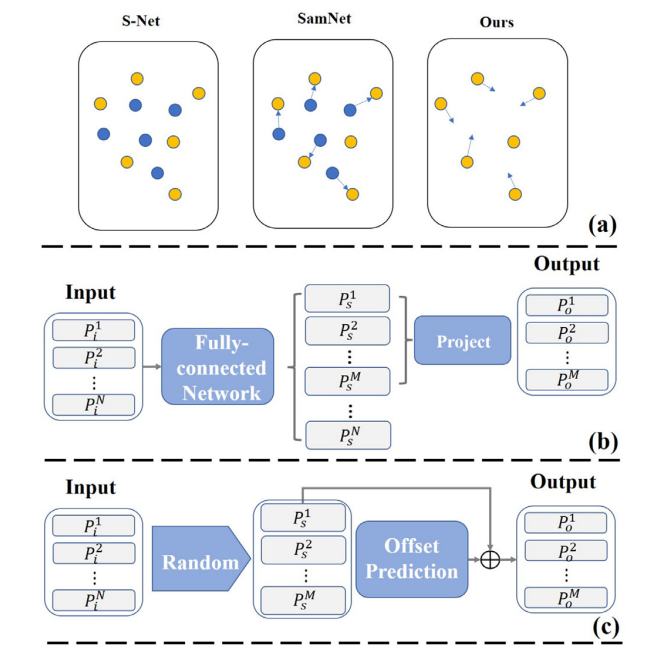
\includegraphics[scale=0.5]{image1}
\caption{(a) shows the differences between learning-based sampling strategies, while (b) and (c) present the discrepancy between progress-net and our method in multiresolution sampling}
\label{fig:fig1}
\end{figure}

Our contributions can be summarized as:
\begin{itemize}
	\item We propose a novel learning-based point cloud sampling
framework named fast sampling network (FPN) by driving existing randomly sampled points to better positions;
    \item We introduce a hybrid training strategy to help FPN adapt to
different sampling resolutions by randomly introducing selecting the resolution of initial points during training;
\end{itemize}

\section{Methodology}
\subsection{Basic Pipeline}
The basic pipeline of FPN is presented in Fig. 2. We aggregate global features from the input points with a set of multilevel perceptions (MLPs) and Max Pooling following PointNet \cite{qi2017pointnet}.
\subsection{Hybrid Training Strategy}
The achievement of HTS is presented as Algorithm 9.
\subsection{Loss function}
The range constraint can be presented as
\begin{equation}
	\mathcal{L}_{rc}=\frac{1}{N}\sum||S_o-S_i||_2
\end{equation}

For reconstructionrelated tasks, it may be Chamfer Distance or Earth Mover Distance [22] defined as\\

\raggedright{$\mathcal{L}_{task}=L_{CD}(S_1,S_2)$}
\begin{equation}
	=\frac{1}{2}\Biggl(\frac{1}{|S_1|}\sum_{x\in S_1} min_{y\in S_2})||x-y||_2+\frac{1}{|S_2|}\sum_{x\in S_2}min_{y\in S_1}||x-y||_2\Biggr)
\end{equation}
or
\begin{equation}
	\mathcal{L}_{task}=\mathcal{L}_{EMD}(S_1,S_2)=min_{\phi ;S_1\rightarrow S_2}\frac{1}{|s_1|}\sum_{x \in S_1}||x-\Phi(x)||_2
\end{equation}

\section{Experiments}
\begin{table}
    \centering
    \begin{tabular}{cccc}
    	&$f_1$&$f_2$&$f_3$\\

    \end{tabular}

\end{table}



\printbibliography
\end{multicols}

\end{document}
